\documentclass[twoside]{book}

% Packages required by doxygen
\usepackage{fixltx2e}
\usepackage{calc}
\usepackage{doxygen}
\usepackage[export]{adjustbox} % also loads graphicx
\usepackage{graphicx}
\usepackage[utf8]{inputenc}
\usepackage{makeidx}
\usepackage{multicol}
\usepackage{multirow}
\PassOptionsToPackage{warn}{textcomp}
\usepackage{textcomp}
\usepackage[nointegrals]{wasysym}
\usepackage[table]{xcolor}

% Font selection
\usepackage[T1]{fontenc}
\usepackage[scaled=.90]{helvet}
\usepackage{courier}
\usepackage{amssymb}
\usepackage{sectsty}
\renewcommand{\familydefault}{\sfdefault}
\allsectionsfont{%
  \fontseries{bc}\selectfont%
  \color{darkgray}%
}
\renewcommand{\DoxyLabelFont}{%
  \fontseries{bc}\selectfont%
  \color{darkgray}%
}
\newcommand{\+}{\discretionary{\mbox{\scriptsize$\hookleftarrow$}}{}{}}

% Page & text layout
\usepackage{geometry}
\geometry{%
  a4paper,%
  top=2.5cm,%
  bottom=2.5cm,%
  left=2.5cm,%
  right=2.5cm%
}
\tolerance=750
\hfuzz=15pt
\hbadness=750
\setlength{\emergencystretch}{15pt}
\setlength{\parindent}{0cm}
\setlength{\parskip}{3ex plus 2ex minus 2ex}
\makeatletter
\renewcommand{\paragraph}{%
  \@startsection{paragraph}{4}{0ex}{-1.0ex}{1.0ex}{%
    \normalfont\normalsize\bfseries\SS@parafont%
  }%
}
\renewcommand{\subparagraph}{%
  \@startsection{subparagraph}{5}{0ex}{-1.0ex}{1.0ex}{%
    \normalfont\normalsize\bfseries\SS@subparafont%
  }%
}
\makeatother

% Headers & footers
\usepackage{fancyhdr}
\pagestyle{fancyplain}
\fancyhead[LE]{\fancyplain{}{\bfseries\thepage}}
\fancyhead[CE]{\fancyplain{}{}}
\fancyhead[RE]{\fancyplain{}{\bfseries\leftmark}}
\fancyhead[LO]{\fancyplain{}{\bfseries\rightmark}}
\fancyhead[CO]{\fancyplain{}{}}
\fancyhead[RO]{\fancyplain{}{\bfseries\thepage}}
\fancyfoot[LE]{\fancyplain{}{}}
\fancyfoot[CE]{\fancyplain{}{}}
\fancyfoot[RE]{\fancyplain{}{\bfseries\scriptsize Generated by Doxygen }}
\fancyfoot[LO]{\fancyplain{}{\bfseries\scriptsize Generated by Doxygen }}
\fancyfoot[CO]{\fancyplain{}{}}
\fancyfoot[RO]{\fancyplain{}{}}
\renewcommand{\footrulewidth}{0.4pt}
\renewcommand{\chaptermark}[1]{%
  \markboth{#1}{}%
}
\renewcommand{\sectionmark}[1]{%
  \markright{\thesection\ #1}%
}

% Indices & bibliography
\usepackage{natbib}
\usepackage[titles]{tocloft}
\setcounter{tocdepth}{3}
\setcounter{secnumdepth}{5}
\makeindex

% Hyperlinks (required, but should be loaded last)
\usepackage{ifpdf}
\ifpdf
  \usepackage[pdftex,pagebackref=true]{hyperref}
\else
  \usepackage[ps2pdf,pagebackref=true]{hyperref}
\fi
\hypersetup{%
  colorlinks=true,%
  linkcolor=blue,%
  citecolor=blue,%
  unicode%
}

% Custom commands
\newcommand{\clearemptydoublepage}{%
  \newpage{\pagestyle{empty}\cleardoublepage}%
}

\usepackage{caption}
\captionsetup{labelsep=space,justification=centering,font={bf},singlelinecheck=off,skip=4pt,position=top}

%===== C O N T E N T S =====

\begin{document}

% Titlepage & ToC
\hypersetup{pageanchor=false,
             bookmarksnumbered=true,
             pdfencoding=unicode
            }
\pagenumbering{alph}
\begin{titlepage}
\vspace*{7cm}
\begin{center}%
{\Large Geode }\\
\vspace*{1cm}
{\large Generated by Doxygen 1.8.14}\\
\end{center}
\end{titlepage}
\clearemptydoublepage
\pagenumbering{roman}
\tableofcontents
\clearemptydoublepage
\pagenumbering{arabic}
\hypersetup{pageanchor=true}

%--- Begin generated contents ---
\chapter{Todo List}
\label{todo}
\Hypertarget{todo}

\begin{DoxyRefList}
\item[\label{todo__todo000001}%
\Hypertarget{todo__todo000001}%
Class \mbox{\hyperlink{classfeedback__bus}{feedback\+\_\+bus}} ]write docs 
\end{DoxyRefList}
\chapter{Hierarchical Index}
\section{Class Hierarchy}
This inheritance list is sorted roughly, but not completely, alphabetically\+:\begin{DoxyCompactList}
\item \contentsline{section}{axon}{\pageref{classaxon}}{}
\item \contentsline{section}{concurrent\+\_\+neural\+\_\+network}{\pageref{classconcurrent__neural__network}}{}
\item \contentsline{section}{dna}{\pageref{structdna}}{}
\item \contentsline{section}{feedback\+\_\+bus}{\pageref{classfeedback__bus}}{}
\item \contentsline{section}{Genetic\+Algorithm$<$ T $>$}{\pageref{class_genetic_algorithm}}{}
\item \contentsline{section}{neuron}{\pageref{classneuron}}{}
\begin{DoxyCompactList}
\item \contentsline{section}{output\+\_\+neuron}{\pageref{classoutput__neuron}}{}
\end{DoxyCompactList}
\end{DoxyCompactList}

\chapter{Class Index}
\section{Class List}
Here are the classes, structs, unions and interfaces with brief descriptions\+:\begin{DoxyCompactList}
\item\contentsline{section}{\mbox{\hyperlink{classaxon}{axon}} }{\pageref{classaxon}}{}
\item\contentsline{section}{\mbox{\hyperlink{classconcurrent__neural__network}{concurrent\+\_\+neural\+\_\+network}} \\*Representa una red neuronal en formato matriz de costes }{\pageref{classconcurrent__neural__network}}{}
\item\contentsline{section}{\mbox{\hyperlink{structdna}{dna}} \\*Estructura que representa un genoma de red neuronal }{\pageref{structdna}}{}
\item\contentsline{section}{\mbox{\hyperlink{classfeedback__bus}{feedback\+\_\+bus}} \\*Similar to \mbox{\hyperlink{classneuron}{neuron}}, it allow cycles (feedback) between neurons by capturing de feedback data and propagate it after regular forward data propagation have ended }{\pageref{classfeedback__bus}}{}
\item\contentsline{section}{\mbox{\hyperlink{class_genetic_algorithm}{Genetic\+Algorithm$<$ T $>$}} \\*Framework parametrizado para el manejo de algoritmos genéticos. Este sistema trata de abstraer al programador de los procesos relacionados con el algoritmo realizando las operaciones de cruce, mutación y evaluación por él según sea conveniente }{\pageref{class_genetic_algorithm}}{}
\item\contentsline{section}{\mbox{\hyperlink{classneuron}{neuron}} \\*Perceptron like neuron }{\pageref{classneuron}}{}
\item\contentsline{section}{\mbox{\hyperlink{classoutput__neuron}{output\+\_\+neuron}} \\*Neuron that check if have any input axon before trying to calculate its output. If have none it outputs 0 }{\pageref{classoutput__neuron}}{}
\end{DoxyCompactList}

\chapter{Class Documentation}
\hypertarget{classaxon}{}\section{axon Class Reference}
\label{classaxon}\index{axon@{axon}}
\subsection*{Public Member Functions}
\begin{DoxyCompactItemize}
\item 
\mbox{\Hypertarget{classaxon_a43c15789a30c17884094ec0fa1905958}\label{classaxon_a43c15789a30c17884094ec0fa1905958}} 
{\bfseries axon} (double w)
\item 
\mbox{\Hypertarget{classaxon_aaba6ceea9994fe5e18dc6f71f8a662ee}\label{classaxon_aaba6ceea9994fe5e18dc6f71f8a662ee}} 
void {\bfseries set\+\_\+value} (double v)
\item 
\mbox{\Hypertarget{classaxon_a0c7d1068cc20ceec501edd225b17335d}\label{classaxon_a0c7d1068cc20ceec501edd225b17335d}} 
double {\bfseries get\+\_\+value} () const
\end{DoxyCompactItemize}


\subsection{Detailed Description}


Definition at line 22 of file axon.\+h.



The documentation for this class was generated from the following file\+:\begin{DoxyCompactItemize}
\item 
backend/neural\+\_\+network/axon.\+h\end{DoxyCompactItemize}

\hypertarget{classconcurrent__neural__network}{}\section{concurrent\+\_\+neural\+\_\+network Class Reference}
\label{classconcurrent__neural__network}\index{concurrent\+\_\+neural\+\_\+network@{concurrent\+\_\+neural\+\_\+network}}


Representa una red neuronal en formato matriz de costes.  




{\ttfamily \#include $<$concurrent\+\_\+neural\+\_\+network.\+h$>$}

\subsection*{Public Member Functions}
\begin{DoxyCompactItemize}
\item 
\mbox{\Hypertarget{classconcurrent__neural__network_a3380e6a7b4575fd5131c5af31c8bbaf1}\label{classconcurrent__neural__network_a3380e6a7b4575fd5131c5af31c8bbaf1}} 
{\bfseries concurrent\+\_\+neural\+\_\+network} (const std\+::vector$<$ std\+::vector$<$ std\+::pair$<$ bool, T\+Y\+PE $>$$>$$>$ \&cost, unsigned inputs, unsigned ouputs)
\item 
\mbox{\hyperlink{classconcurrent__neural__network_ae6b889b695e5959b4265653235d54971}{concurrent\+\_\+neural\+\_\+network}} (unsigned n\+\_\+neurons, unsigned input, unsigned output)
\begin{DoxyCompactList}\small\item\em Random values default constructor. \end{DoxyCompactList}\item 
\mbox{\Hypertarget{classconcurrent__neural__network_ac3e8b9ff79be67ed0a102bc4b05bbb86}\label{classconcurrent__neural__network_ac3e8b9ff79be67ed0a102bc4b05bbb86}} 
{\bfseries concurrent\+\_\+neural\+\_\+network} (const \mbox{\hyperlink{classconcurrent__neural__network}{concurrent\+\_\+neural\+\_\+network}} \&aux)
\item 
\mbox{\hyperlink{classconcurrent__neural__network_af59e6e4b876ebb11c7a41b42bed935de}{concurrent\+\_\+neural\+\_\+network}} (const \mbox{\hyperlink{structdna}{dna}} \&D\+NA)
\begin{DoxyCompactList}\small\item\em Genera la red neuronal a partir de un adn válido, según la codificación contemplada en \mbox{\hyperlink{structdna}{dna}}. \end{DoxyCompactList}\item 
\mbox{\hyperlink{structdna}{dna}} \mbox{\hyperlink{classconcurrent__neural__network_a1301ba2e3c5d21633df37d1ab6ae7bb8}{to\+\_\+dna}} ()
\begin{DoxyCompactList}\small\item\em Genera un adn que codifique la información de la red neuronal contenida. \end{DoxyCompactList}\item 
\mbox{\Hypertarget{classconcurrent__neural__network_a6aceadc0feff8c47cec4423041096c97}\label{classconcurrent__neural__network_a6aceadc0feff8c47cec4423041096c97}} 
void {\bfseries operator=} (const \mbox{\hyperlink{classconcurrent__neural__network}{concurrent\+\_\+neural\+\_\+network}} \&aux)
\item 
\mbox{\Hypertarget{classconcurrent__neural__network_a23841b7f99d68cde6242b1468e4e025d}\label{classconcurrent__neural__network_a23841b7f99d68cde6242b1468e4e025d}} 
std\+::vector$<$ std\+::vector$<$ T\+Y\+PE $>$ $>$ {\bfseries get\+\_\+cost\+\_\+matrix} () const
\item 
\mbox{\Hypertarget{classconcurrent__neural__network_ae988d079e4f402c1b28b6634339cfaa7}\label{classconcurrent__neural__network_ae988d079e4f402c1b28b6634339cfaa7}} 
std\+::vector$<$ std\+::vector$<$ bool $>$ $>$ {\bfseries get\+\_\+graph\+\_\+matrix} () const
\item 
bool \mbox{\hyperlink{classconcurrent__neural__network_ab3df0ad8df7bb93cc3caca1d0e28e79f}{calculate}} (std\+::vector$<$ double $>$ \&input\+\_\+values, std\+::vector$<$ double $>$ \&output\+\_\+values)
\begin{DoxyCompactList}\small\item\em Calcula la respuesta de la red neuronal ante una entrada. \end{DoxyCompactList}\item 
\mbox{\Hypertarget{classconcurrent__neural__network_a0e1cdef29d52edde39808ce54bb309a9}\label{classconcurrent__neural__network_a0e1cdef29d52edde39808ce54bb309a9}} 
void \mbox{\hyperlink{classconcurrent__neural__network_a0e1cdef29d52edde39808ce54bb309a9}{print}} () const
\begin{DoxyCompactList}\small\item\em Imprime la red neuronal como matriz de costes. \end{DoxyCompactList}\item 
\mbox{\Hypertarget{classconcurrent__neural__network_a91262b8a313f2bdf96472221197b7d12}\label{classconcurrent__neural__network_a91262b8a313f2bdf96472221197b7d12}} 
unsigned {\bfseries c\+\_\+steps} ()
\end{DoxyCompactItemize}


\subsection{Detailed Description}
Representa una red neuronal en formato matriz de costes. 

Definition at line 44 of file concurrent\+\_\+neural\+\_\+network.\+h.



\subsection{Constructor \& Destructor Documentation}
\mbox{\Hypertarget{classconcurrent__neural__network_ae6b889b695e5959b4265653235d54971}\label{classconcurrent__neural__network_ae6b889b695e5959b4265653235d54971}} 
\index{concurrent\+\_\+neural\+\_\+network@{concurrent\+\_\+neural\+\_\+network}!concurrent\+\_\+neural\+\_\+network@{concurrent\+\_\+neural\+\_\+network}}
\index{concurrent\+\_\+neural\+\_\+network@{concurrent\+\_\+neural\+\_\+network}!concurrent\+\_\+neural\+\_\+network@{concurrent\+\_\+neural\+\_\+network}}
\subsubsection{\texorpdfstring{concurrent\+\_\+neural\+\_\+network()}{concurrent\_neural\_network()}\hspace{0.1cm}{\footnotesize\ttfamily [1/2]}}
{\footnotesize\ttfamily concurrent\+\_\+neural\+\_\+network\+::concurrent\+\_\+neural\+\_\+network (\begin{DoxyParamCaption}\item[{unsigned}]{n\+\_\+neurons,  }\item[{unsigned}]{input,  }\item[{unsigned}]{output }\end{DoxyParamCaption})\hspace{0.3cm}{\ttfamily [explicit]}}



Random values default constructor. 


\begin{DoxyParams}{Parameters}
{\em n\+\_\+neurons} & p\+\_\+n\+\_\+neurons\+:... \\
\hline
{\em input} & p\+\_\+input\+:... \\
\hline
{\em output} & \$\{p\+\_\+output\+:...\} \\
\hline
\end{DoxyParams}


Definition at line 47 of file concurrent\+\_\+neural\+\_\+network.\+cpp.

\mbox{\Hypertarget{classconcurrent__neural__network_af59e6e4b876ebb11c7a41b42bed935de}\label{classconcurrent__neural__network_af59e6e4b876ebb11c7a41b42bed935de}} 
\index{concurrent\+\_\+neural\+\_\+network@{concurrent\+\_\+neural\+\_\+network}!concurrent\+\_\+neural\+\_\+network@{concurrent\+\_\+neural\+\_\+network}}
\index{concurrent\+\_\+neural\+\_\+network@{concurrent\+\_\+neural\+\_\+network}!concurrent\+\_\+neural\+\_\+network@{concurrent\+\_\+neural\+\_\+network}}
\subsubsection{\texorpdfstring{concurrent\+\_\+neural\+\_\+network()}{concurrent\_neural\_network()}\hspace{0.1cm}{\footnotesize\ttfamily [2/2]}}
{\footnotesize\ttfamily concurrent\+\_\+neural\+\_\+network\+::concurrent\+\_\+neural\+\_\+network (\begin{DoxyParamCaption}\item[{const \mbox{\hyperlink{structdna}{dna}} \&}]{D\+NA }\end{DoxyParamCaption})}



Genera la red neuronal a partir de un adn válido, según la codificación contemplada en \mbox{\hyperlink{structdna}{dna}}. 


\begin{DoxyParams}{Parameters}
{\em dna} & adn empleado para la construcción \\
\hline
\end{DoxyParams}


Definition at line 78 of file concurrent\+\_\+neural\+\_\+network.\+cpp.



\subsection{Member Function Documentation}
\mbox{\Hypertarget{classconcurrent__neural__network_ab3df0ad8df7bb93cc3caca1d0e28e79f}\label{classconcurrent__neural__network_ab3df0ad8df7bb93cc3caca1d0e28e79f}} 
\index{concurrent\+\_\+neural\+\_\+network@{concurrent\+\_\+neural\+\_\+network}!calculate@{calculate}}
\index{calculate@{calculate}!concurrent\+\_\+neural\+\_\+network@{concurrent\+\_\+neural\+\_\+network}}
\subsubsection{\texorpdfstring{calculate()}{calculate()}}
{\footnotesize\ttfamily bool concurrent\+\_\+neural\+\_\+network\+::calculate (\begin{DoxyParamCaption}\item[{std\+::vector$<$ double $>$ \&}]{input\+\_\+values,  }\item[{std\+::vector$<$ double $>$ \&}]{output\+\_\+values }\end{DoxyParamCaption})}



Calcula la respuesta de la red neuronal ante una entrada. 


\begin{DoxyParams}{Parameters}
{\em inputs} & Datos con los que se alimenta a las neuronas de entrada \\
\hline
{\em outputs} & Contendrá los resultados de las neuronas de salida tras la operación \\
\hline
\end{DoxyParams}


Definition at line 230 of file concurrent\+\_\+neural\+\_\+network.\+cpp.

\mbox{\Hypertarget{classconcurrent__neural__network_a1301ba2e3c5d21633df37d1ab6ae7bb8}\label{classconcurrent__neural__network_a1301ba2e3c5d21633df37d1ab6ae7bb8}} 
\index{concurrent\+\_\+neural\+\_\+network@{concurrent\+\_\+neural\+\_\+network}!to\+\_\+dna@{to\+\_\+dna}}
\index{to\+\_\+dna@{to\+\_\+dna}!concurrent\+\_\+neural\+\_\+network@{concurrent\+\_\+neural\+\_\+network}}
\subsubsection{\texorpdfstring{to\+\_\+dna()}{to\_dna()}}
{\footnotesize\ttfamily \mbox{\hyperlink{structdna}{dna}} concurrent\+\_\+neural\+\_\+network\+::to\+\_\+dna (\begin{DoxyParamCaption}{ }\end{DoxyParamCaption})}



Genera un adn que codifique la información de la red neuronal contenida. 

\begin{DoxyReturn}{Returns}
dna Adn con la información de la red neuronal. 
\end{DoxyReturn}


Definition at line 190 of file concurrent\+\_\+neural\+\_\+network.\+cpp.



The documentation for this class was generated from the following files\+:\begin{DoxyCompactItemize}
\item 
backend/neural\+\_\+network/concurrent\+\_\+neural\+\_\+network.\+h\item 
backend/neural\+\_\+network/concurrent\+\_\+neural\+\_\+network.\+cpp\end{DoxyCompactItemize}

\hypertarget{structdna}{}\section{dna Struct Reference}
\label{structdna}\index{dna@{dna}}


Estructura que representa un genoma de red neuronal.  




{\ttfamily \#include $<$dna.\+h$>$}

\subsection*{Public Member Functions}
\begin{DoxyCompactItemize}
\item 
\mbox{\Hypertarget{structdna_a54a35c5c7c03a95a4b2d0e1c1513ddba}\label{structdna_a54a35c5c7c03a95a4b2d0e1c1513ddba}} 
{\bfseries dna} (const \mbox{\hyperlink{structdna}{dna}} \&D\+NA)
\item 
\mbox{\Hypertarget{structdna_a1ba2ef3fbc06a7307edb8dfa6d01187b}\label{structdna_a1ba2ef3fbc06a7307edb8dfa6d01187b}} 
{\bfseries dna} (char $\ast$s, unsigned b, unsigned i, unsigned o)
\item 
\mbox{\Hypertarget{structdna_a07c485849dfec41e9d5a8873aaa61296}\label{structdna_a07c485849dfec41e9d5a8873aaa61296}} 
void {\bfseries operator=} (const \mbox{\hyperlink{structdna}{dna}} \&aux)
\end{DoxyCompactItemize}
\subsection*{Public Attributes}
\begin{DoxyCompactItemize}
\item 
char $\ast$ \mbox{\hyperlink{structdna_aed2989af9e06a398429aca34de0d3b3f}{sequence}}
\begin{DoxyCompactList}\small\item\em Secuencia {\itshape binaria} que contiene toda la información para generar la red neuronal. Codifica dos matrices de tamaño n x n donde n es el número de neuronas y las matrices corresponden a\+: \end{DoxyCompactList}\item 
\mbox{\Hypertarget{structdna_a57e280bcf988165eb8692ecda1967230}\label{structdna_a57e280bcf988165eb8692ecda1967230}} 
unsigned \mbox{\hyperlink{structdna_a57e280bcf988165eb8692ecda1967230}{byte\+\_\+sz}}
\begin{DoxyCompactList}\small\item\em Tamaño en bytes de la cadena contenida en \mbox{\hyperlink{structdna_aed2989af9e06a398429aca34de0d3b3f}{sequence}}. \end{DoxyCompactList}\item 
\mbox{\Hypertarget{structdna_a8fbd61efb3a087665efb344333c724dc}\label{structdna_a8fbd61efb3a087665efb344333c724dc}} 
unsigned \mbox{\hyperlink{structdna_a8fbd61efb3a087665efb344333c724dc}{input\+\_\+neurons}}
\begin{DoxyCompactList}\small\item\em Número de neuronas de entrada, las neuronas desde 0 hasta \mbox{\hyperlink{structdna_a8fbd61efb3a087665efb344333c724dc}{input\+\_\+neurons}} se consideran neuronas de entrada. Primeras \mbox{\hyperlink{structdna_a8fbd61efb3a087665efb344333c724dc}{input\+\_\+neurons}} neuronas. \end{DoxyCompactList}\item 
\mbox{\Hypertarget{structdna_a8939224e5ff137b49f031dfb649b2068}\label{structdna_a8939224e5ff137b49f031dfb649b2068}} 
unsigned \mbox{\hyperlink{structdna_a8939224e5ff137b49f031dfb649b2068}{output\+\_\+neurons}}
\begin{DoxyCompactList}\small\item\em Número de neuronas de salida, las neuronas desde (n -\/ \mbox{\hyperlink{structdna_a8939224e5ff137b49f031dfb649b2068}{output\+\_\+neurons}}) hasta n se consideran neuronas de entrada. Últimas \mbox{\hyperlink{structdna_a8939224e5ff137b49f031dfb649b2068}{output\+\_\+neurons}} neuronas. \end{DoxyCompactList}\end{DoxyCompactItemize}


\subsection{Detailed Description}
Estructura que representa un genoma de red neuronal. 

Definition at line 13 of file dna.\+h.



\subsection{Member Data Documentation}
\mbox{\Hypertarget{structdna_aed2989af9e06a398429aca34de0d3b3f}\label{structdna_aed2989af9e06a398429aca34de0d3b3f}} 
\index{dna@{dna}!sequence@{sequence}}
\index{sequence@{sequence}!dna@{dna}}
\subsubsection{\texorpdfstring{sequence}{sequence}}
{\footnotesize\ttfamily char$\ast$ dna\+::sequence}



Secuencia {\itshape binaria} que contiene toda la información para generar la red neuronal. Codifica dos matrices de tamaño n x n donde n es el número de neuronas y las matrices corresponden a\+: 

Matriz a\+: matriz booleana, indica si existe un determinado axón que ij que conecta la neurona i con la neurona j. En el caso de i = j es indiferente el valor.

Matriz b\+: matriz de costes, indica el peso del axón ij en caso de existir. En el caso de i = j el valor representa el umbral.

La codificación es la siguiente, por orden de aparición de los elementos\+:

n \+: número de neuronas. 4 bytes a00 \+: trivial, una neurona siempre conecta consigo misma b00 \+: valor del umbral de la neurona 0 a01 \+: existencia o no de un axón que conecte la neurona 0 con la 1 b01 \+: peso del axón que conecta la neurona 0 con la 1 ... ann \+: trivial, una neurona siempre conecta consigo misma bnn \+: valor del umbral de la neurona n 

Definition at line 37 of file dna.\+h.



The documentation for this struct was generated from the following files\+:\begin{DoxyCompactItemize}
\item 
backend/neural\+\_\+network/dna.\+h\item 
backend/neural\+\_\+network/dna.\+cpp\end{DoxyCompactItemize}

\hypertarget{classfeedback__bus}{}\section{feedback\+\_\+bus Class Reference}
\label{classfeedback__bus}\index{feedback\+\_\+bus@{feedback\+\_\+bus}}


Similar to \mbox{\hyperlink{classneuron}{neuron}}, it allow cycles (feedback) between neurons by capturing de feedback data and propagate it after regular forward data propagation have ended.  




{\ttfamily \#include $<$feedback\+\_\+bus.\+h$>$}

\subsection*{Public Member Functions}
\begin{DoxyCompactItemize}
\item 
\mbox{\Hypertarget{classfeedback__bus_a0eab17d3da687177bae330941752e4d5}\label{classfeedback__bus_a0eab17d3da687177bae330941752e4d5}} 
{\bfseries feedback\+\_\+bus} (\mbox{\hyperlink{classneuron}{neuron}} $\ast$des)
\item 
\mbox{\Hypertarget{classfeedback__bus_a6d092b9d2e3868f0780dd75ddf0c35ac}\label{classfeedback__bus_a6d092b9d2e3868f0780dd75ddf0c35ac}} 
void {\bfseries add\+\_\+connection} (\mbox{\hyperlink{classneuron}{neuron}} $\ast$origin, double weight)
\item 
\mbox{\Hypertarget{classfeedback__bus_aa26c71125fe3bc234aad9c7d21a069ce}\label{classfeedback__bus_aa26c71125fe3bc234aad9c7d21a069ce}} 
void {\bfseries propagate\+\_\+value} ()
\end{DoxyCompactItemize}


\subsection{Detailed Description}
Similar to \mbox{\hyperlink{classneuron}{neuron}}, it allow cycles (feedback) between neurons by capturing de feedback data and propagate it after regular forward data propagation have ended. 

\begin{DoxyRefDesc}{Todo}
\item[\mbox{\hyperlink{todo__todo000001}{Todo}}]write docs \end{DoxyRefDesc}


Definition at line 33 of file feedback\+\_\+bus.\+h.



The documentation for this class was generated from the following files\+:\begin{DoxyCompactItemize}
\item 
backend/neural\+\_\+network/feedback\+\_\+bus.\+h\item 
backend/neural\+\_\+network/feedback\+\_\+bus.\+cpp\end{DoxyCompactItemize}

\hypertarget{class_genetic_algorithm}{}\section{Genetic\+Algorithm$<$ T $>$ Class Template Reference}
\label{class_genetic_algorithm}\index{Genetic\+Algorithm$<$ T $>$@{Genetic\+Algorithm$<$ T $>$}}


Framework parametrizado para el manejo de algoritmos genéticos. Este sistema trata de abstraer al programador de los procesos relacionados con el algoritmo realizando las operaciones de cruce, mutación y evaluación por él según sea conveniente.  




{\ttfamily \#include $<$geneticalgorithm.\+h$>$}

\subsection*{Public Member Functions}
\begin{DoxyCompactItemize}
\item 
\mbox{\Hypertarget{class_genetic_algorithm_a6ca0bbf76e60cacdd77712971dded001}\label{class_genetic_algorithm_a6ca0bbf76e60cacdd77712971dded001}} 
std\+::vector$<$ T $>$ {\bfseries get\+\_\+best\+\_\+candidates} ()
\item 
\mbox{\hyperlink{class_genetic_algorithm_a9fda0f2f53ba15c4dc932d37eab9aff7}{Genetic\+Algorithm}} (std\+::function$<$ T(T \&, T \&)$>$ operator\+\_\+cross, std\+::function$<$ void(T \&, unsigned)$>$ operator\+\_\+mutate, std\+::function$<$ double(const T \&)$>$ operator\+\_\+evaluator, unsigned population\+\_\+s, unsigned candidates\+\_\+s, unsigned mutation\+\_\+r)
\begin{DoxyCompactList}\small\item\em Constructor del algoritmo genético. \end{DoxyCompactList}\item 
void \mbox{\hyperlink{class_genetic_algorithm_a9e3afa46dbfb501b42e1905023b47432}{set\+\_\+population\+\_\+parameters}} (unsigned population\+\_\+s, unsigned candidates\+\_\+s, unsigned mutation\+\_\+r)
\begin{DoxyCompactList}\small\item\em Adjust parameters of the simulation any time. \end{DoxyCompactList}\item 
bool \mbox{\hyperlink{class_genetic_algorithm_a5d4afa4cd644ae80b6001184f6b8728d}{step}} ()
\begin{DoxyCompactList}\small\item\em Simulates a complete generation. (Create population, mutate it, evaluate it, generate new one) \end{DoxyCompactList}\item 
\mbox{\Hypertarget{class_genetic_algorithm_ab52124a783d776e8ba658bf665e0be66}\label{class_genetic_algorithm_ab52124a783d776e8ba658bf665e0be66}} 
void \mbox{\hyperlink{class_genetic_algorithm_ab52124a783d776e8ba658bf665e0be66}{semi\+\_\+step}} ()
\begin{DoxyCompactList}\small\item\em Makes the simulation advance half step by generatin a new population and mutate it. \mbox{\hyperlink{class_genetic_algorithm_af1632165d5b43d91b290a8a257e0f0e7}{set\+\_\+external\+\_\+evaluations}} should be used to complete the iteration. \end{DoxyCompactList}\item 
\mbox{\Hypertarget{class_genetic_algorithm_a3265574d1fe7cbe5975ca55ac15cb3d7}\label{class_genetic_algorithm_a3265574d1fe7cbe5975ca55ac15cb3d7}} 
std\+::vector$<$ T $>$ {\bfseries get\+\_\+population} ()
\item 
void \mbox{\hyperlink{class_genetic_algorithm_af1632165d5b43d91b290a8a257e0f0e7}{set\+\_\+external\+\_\+evaluations}} (std\+::vector$<$ double $>$ evaluations)
\begin{DoxyCompactList}\small\item\em Sets a external evaluation for each individiual. Completes the second half of the iteration, initiated by \mbox{\hyperlink{class_genetic_algorithm_ab52124a783d776e8ba658bf665e0be66}{semi\+\_\+step}}. \end{DoxyCompactList}\item 
void \mbox{\hyperlink{class_genetic_algorithm_a5ed6d3f823943638e0c3688fdf788e1c}{set\+\_\+initial\+\_\+population}} (const std\+::vector$<$ T $>$ \&i\+\_\+population)
\begin{DoxyCompactList}\small\item\em Sets the initial population of the simulation. Automatically adjust the size to accomplish with the one seted in \mbox{\hyperlink{class_genetic_algorithm}{Genetic\+Algorithm}} or \#set\+\_\+poblation\+\_\+parameters by copy / delete elements. \end{DoxyCompactList}\item 
\mbox{\Hypertarget{class_genetic_algorithm_a062f45c41d1f652e2f1794a06e8ba161}\label{class_genetic_algorithm_a062f45c41d1f652e2f1794a06e8ba161}} 
void \mbox{\hyperlink{class_genetic_algorithm_a062f45c41d1f652e2f1794a06e8ba161}{print\+\_\+best}} ()
\begin{DoxyCompactList}\small\item\em Print the best candidates and its score. \end{DoxyCompactList}\end{DoxyCompactItemize}


\subsection{Detailed Description}
\subsubsection*{template$<$class T$>$\newline
class Genetic\+Algorithm$<$ T $>$}

Framework parametrizado para el manejo de algoritmos genéticos. Este sistema trata de abstraer al programador de los procesos relacionados con el algoritmo realizando las operaciones de cruce, mutación y evaluación por él según sea conveniente. 

El programador debe proporcionar no obstante 3 funciones que definan estos operadores para los individuos de tipo \#T con los que se emplearán.

La generación de población y su mutación se realiza de forma concurrente, asignándole un hilo a cada individuo. 

Definition at line 25 of file geneticalgorithm.\+h.



\subsection{Constructor \& Destructor Documentation}
\mbox{\Hypertarget{class_genetic_algorithm_a9fda0f2f53ba15c4dc932d37eab9aff7}\label{class_genetic_algorithm_a9fda0f2f53ba15c4dc932d37eab9aff7}} 
\index{Genetic\+Algorithm@{Genetic\+Algorithm}!Genetic\+Algorithm@{Genetic\+Algorithm}}
\index{Genetic\+Algorithm@{Genetic\+Algorithm}!Genetic\+Algorithm@{Genetic\+Algorithm}}
\subsubsection{\texorpdfstring{Genetic\+Algorithm()}{GeneticAlgorithm()}}
{\footnotesize\ttfamily template$<$class T$>$ \\
\mbox{\hyperlink{class_genetic_algorithm}{Genetic\+Algorithm}}$<$ T $>$\+::\mbox{\hyperlink{class_genetic_algorithm}{Genetic\+Algorithm}} (\begin{DoxyParamCaption}\item[{std\+::function$<$ T(T \&, T \&)$>$}]{operator\+\_\+cross,  }\item[{std\+::function$<$ void(T \&, unsigned)$>$}]{operator\+\_\+mutate,  }\item[{std\+::function$<$ double(const T \&)$>$}]{operator\+\_\+evaluator,  }\item[{unsigned}]{population\+\_\+s,  }\item[{unsigned}]{candidates\+\_\+s,  }\item[{unsigned}]{mutation\+\_\+r }\end{DoxyParamCaption})\hspace{0.3cm}{\ttfamily [inline]}, {\ttfamily [explicit]}}



Constructor del algoritmo genético. 


\begin{DoxyParams}{Parameters}
{\em operator\+\_\+cross} & Función lambda que expecifica de qué manera han de cruzarse los genomas de individuos \#T \\
\hline
{\em operator\+\_\+mutate} & Función lambda que expecifica de qué manera han de mutarse los genomas de individuos \#T \\
\hline
{\em operator\+\_\+evalautor} & Función lambda que expecifica de qué manera han de compararse (función fitness) los genomas de individuos \#T \\
\hline
{\em population\+\_\+s} & Tamaño de la población generada en cada iteración por medio de cruces \\
\hline
{\em candidates\+\_\+s} & Tamaño de la muestra seleccionada por la función evaluadora. \\
\hline
\end{DoxyParams}


Definition at line 146 of file geneticalgorithm.\+h.



\subsection{Member Function Documentation}
\mbox{\Hypertarget{class_genetic_algorithm_af1632165d5b43d91b290a8a257e0f0e7}\label{class_genetic_algorithm_af1632165d5b43d91b290a8a257e0f0e7}} 
\index{Genetic\+Algorithm@{Genetic\+Algorithm}!set\+\_\+external\+\_\+evaluations@{set\+\_\+external\+\_\+evaluations}}
\index{set\+\_\+external\+\_\+evaluations@{set\+\_\+external\+\_\+evaluations}!Genetic\+Algorithm@{Genetic\+Algorithm}}
\subsubsection{\texorpdfstring{set\+\_\+external\+\_\+evaluations()}{set\_external\_evaluations()}}
{\footnotesize\ttfamily template$<$class T$>$ \\
void \mbox{\hyperlink{class_genetic_algorithm}{Genetic\+Algorithm}}$<$ T $>$\+::set\+\_\+external\+\_\+evaluations (\begin{DoxyParamCaption}\item[{std\+::vector$<$ double $>$}]{evaluations }\end{DoxyParamCaption})\hspace{0.3cm}{\ttfamily [inline]}}



Sets a external evaluation for each individiual. Completes the second half of the iteration, initiated by \mbox{\hyperlink{class_genetic_algorithm_ab52124a783d776e8ba658bf665e0be66}{semi\+\_\+step}}. 


\begin{DoxyParams}{Parameters}
{\em evaluations} & p\+\_\+evaluations\+: Should have the same size as the population. Each i element contains the score of the i individual from population. \\
\hline
\end{DoxyParams}


Definition at line 220 of file geneticalgorithm.\+h.

\mbox{\Hypertarget{class_genetic_algorithm_a5ed6d3f823943638e0c3688fdf788e1c}\label{class_genetic_algorithm_a5ed6d3f823943638e0c3688fdf788e1c}} 
\index{Genetic\+Algorithm@{Genetic\+Algorithm}!set\+\_\+initial\+\_\+population@{set\+\_\+initial\+\_\+population}}
\index{set\+\_\+initial\+\_\+population@{set\+\_\+initial\+\_\+population}!Genetic\+Algorithm@{Genetic\+Algorithm}}
\subsubsection{\texorpdfstring{set\+\_\+initial\+\_\+population()}{set\_initial\_population()}}
{\footnotesize\ttfamily template$<$class T$>$ \\
void \mbox{\hyperlink{class_genetic_algorithm}{Genetic\+Algorithm}}$<$ T $>$\+::set\+\_\+initial\+\_\+population (\begin{DoxyParamCaption}\item[{const std\+::vector$<$ T $>$ \&}]{i\+\_\+population }\end{DoxyParamCaption})\hspace{0.3cm}{\ttfamily [inline]}}



Sets the initial population of the simulation. Automatically adjust the size to accomplish with the one seted in \mbox{\hyperlink{class_genetic_algorithm}{Genetic\+Algorithm}} or \#set\+\_\+poblation\+\_\+parameters by copy / delete elements. 


\begin{DoxyParams}{Parameters}
{\em i\+\_\+population} & population \\
\hline
\end{DoxyParams}


Definition at line 232 of file geneticalgorithm.\+h.

\mbox{\Hypertarget{class_genetic_algorithm_a9e3afa46dbfb501b42e1905023b47432}\label{class_genetic_algorithm_a9e3afa46dbfb501b42e1905023b47432}} 
\index{Genetic\+Algorithm@{Genetic\+Algorithm}!set\+\_\+population\+\_\+parameters@{set\+\_\+population\+\_\+parameters}}
\index{set\+\_\+population\+\_\+parameters@{set\+\_\+population\+\_\+parameters}!Genetic\+Algorithm@{Genetic\+Algorithm}}
\subsubsection{\texorpdfstring{set\+\_\+population\+\_\+parameters()}{set\_population\_parameters()}}
{\footnotesize\ttfamily template$<$class T$>$ \\
void \mbox{\hyperlink{class_genetic_algorithm}{Genetic\+Algorithm}}$<$ T $>$\+::set\+\_\+population\+\_\+parameters (\begin{DoxyParamCaption}\item[{unsigned}]{population\+\_\+s,  }\item[{unsigned}]{candidates\+\_\+s,  }\item[{unsigned}]{mutation\+\_\+r }\end{DoxyParamCaption})\hspace{0.3cm}{\ttfamily [inline]}}



Adjust parameters of the simulation any time. 


\begin{DoxyParams}{Parameters}
{\em population\+\_\+s} & p\+\_\+population\+\_\+s\+: population size \\
\hline
{\em candidates\+\_\+s} & p\+\_\+candidates\+\_\+s\+: candidates size \\
\hline
{\em mutation\+\_\+r} & p\+\_\+mutation\+\_\+r\+: mutation rate \\
\hline
\end{DoxyParams}


Definition at line 174 of file geneticalgorithm.\+h.

\mbox{\Hypertarget{class_genetic_algorithm_a5d4afa4cd644ae80b6001184f6b8728d}\label{class_genetic_algorithm_a5d4afa4cd644ae80b6001184f6b8728d}} 
\index{Genetic\+Algorithm@{Genetic\+Algorithm}!step@{step}}
\index{step@{step}!Genetic\+Algorithm@{Genetic\+Algorithm}}
\subsubsection{\texorpdfstring{step()}{step()}}
{\footnotesize\ttfamily template$<$class T$>$ \\
bool \mbox{\hyperlink{class_genetic_algorithm}{Genetic\+Algorithm}}$<$ T $>$\+::step (\begin{DoxyParamCaption}{ }\end{DoxyParamCaption})\hspace{0.3cm}{\ttfamily [inline]}}



Simulates a complete generation. (Create population, mutate it, evaluate it, generate new one) 

\begin{DoxyReturn}{Returns}
currently always true 
\end{DoxyReturn}


Definition at line 190 of file geneticalgorithm.\+h.



The documentation for this class was generated from the following file\+:\begin{DoxyCompactItemize}
\item 
backend/genetic\+\_\+algorithm/geneticalgorithm.\+h\end{DoxyCompactItemize}

\hypertarget{classneuron}{}\section{neuron Class Reference}
\label{classneuron}\index{neuron@{neuron}}


Perceptron like neuron.  




{\ttfamily \#include $<$neuron.\+h$>$}

Inheritance diagram for neuron\+:\begin{figure}[H]
\begin{center}
\leavevmode
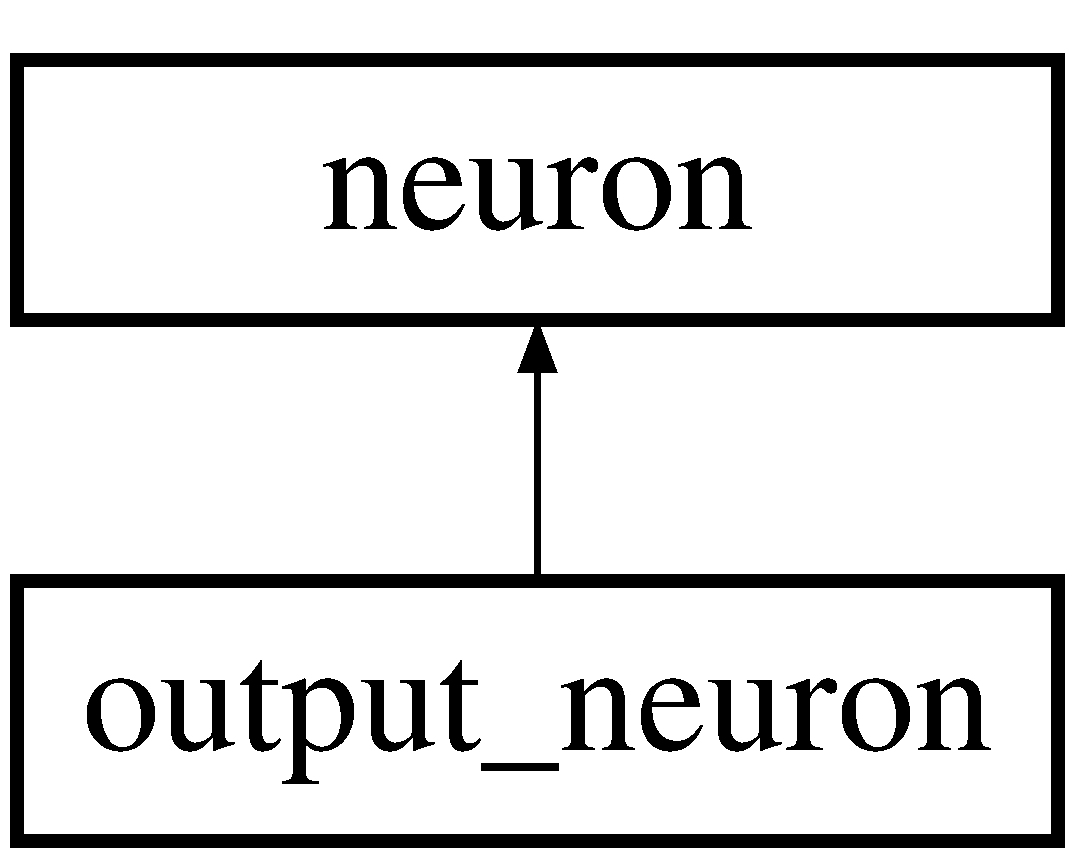
\includegraphics[height=2.000000cm]{classneuron}
\end{center}
\end{figure}
\subsection*{Public Member Functions}
\begin{DoxyCompactItemize}
\item 
\mbox{\Hypertarget{classneuron_afda4f1ba2c739a1c03c407838d1c336a}\label{classneuron_afda4f1ba2c739a1c03c407838d1c336a}} 
void {\bfseries set\+\_\+threshold} (double t)
\item 
\mbox{\Hypertarget{classneuron_a2a88d55500f17c28ae0c262fd5c627f2}\label{classneuron_a2a88d55500f17c28ae0c262fd5c627f2}} 
void {\bfseries add\+\_\+input} (\mbox{\hyperlink{classaxon}{axon}} $\ast$input)
\item 
\mbox{\Hypertarget{classneuron_a5718f629f5bfe73a41f0e3d2f4b6abf0}\label{classneuron_a5718f629f5bfe73a41f0e3d2f4b6abf0}} 
void {\bfseries add\+\_\+output} (\mbox{\hyperlink{classaxon}{axon}} $\ast$output)
\item 
\mbox{\Hypertarget{classneuron_a49f9bb4a8ef9fb8220c66d2ee4752760}\label{classneuron_a49f9bb4a8ef9fb8220c66d2ee4752760}} 
virtual void {\bfseries calculate\+\_\+value} ()
\item 
\mbox{\Hypertarget{classneuron_a697f1ae7d0cb97e66b2382b1f01e47ea}\label{classneuron_a697f1ae7d0cb97e66b2382b1f01e47ea}} 
void {\bfseries propagate\+\_\+value} ()
\item 
\mbox{\Hypertarget{classneuron_a1f560b8ccb0240439df55ac69758ff3d}\label{classneuron_a1f560b8ccb0240439df55ac69758ff3d}} 
double {\bfseries get\+\_\+value} () const
\end{DoxyCompactItemize}
\subsection*{Protected Attributes}
\begin{DoxyCompactItemize}
\item 
\mbox{\Hypertarget{classneuron_a991ef728f717c5421dc1c7eeb239f9a7}\label{classneuron_a991ef728f717c5421dc1c7eeb239f9a7}} 
double {\bfseries value}
\item 
\mbox{\Hypertarget{classneuron_ac730fc8c9d0c6f4d0a26ac9008c5b079}\label{classneuron_ac730fc8c9d0c6f4d0a26ac9008c5b079}} 
double {\bfseries threshold}
\item 
\mbox{\Hypertarget{classneuron_afa18eb496b92d6f3492c585a52562b8a}\label{classneuron_afa18eb496b92d6f3492c585a52562b8a}} 
unsigned {\bfseries n\+\_\+inputs}
\item 
\mbox{\Hypertarget{classneuron_afe6dd27464dcc663c48abfe98b4c3611}\label{classneuron_afe6dd27464dcc663c48abfe98b4c3611}} 
std\+::vector$<$ \mbox{\hyperlink{classaxon}{axon}} $\ast$ $>$ {\bfseries inputs}
\item 
\mbox{\Hypertarget{classneuron_aca8ecff762063d557618a34d7f886390}\label{classneuron_aca8ecff762063d557618a34d7f886390}} 
std\+::vector$<$ \mbox{\hyperlink{classaxon}{axon}} $\ast$ $>$ {\bfseries outputs}
\end{DoxyCompactItemize}


\subsection{Detailed Description}
Perceptron like neuron. 

Definition at line 31 of file neuron.\+h.



The documentation for this class was generated from the following files\+:\begin{DoxyCompactItemize}
\item 
backend/neural\+\_\+network/neuron.\+h\item 
backend/neural\+\_\+network/neuron.\+cpp\end{DoxyCompactItemize}

\hypertarget{classoutput__neuron}{}\section{output\+\_\+neuron Class Reference}
\label{classoutput__neuron}\index{output\+\_\+neuron@{output\+\_\+neuron}}


Neuron that check if have any input axon before trying to calculate its output. If have none it outputs 0.  




{\ttfamily \#include $<$neuron.\+h$>$}

Inheritance diagram for output\+\_\+neuron\+:\begin{figure}[H]
\begin{center}
\leavevmode
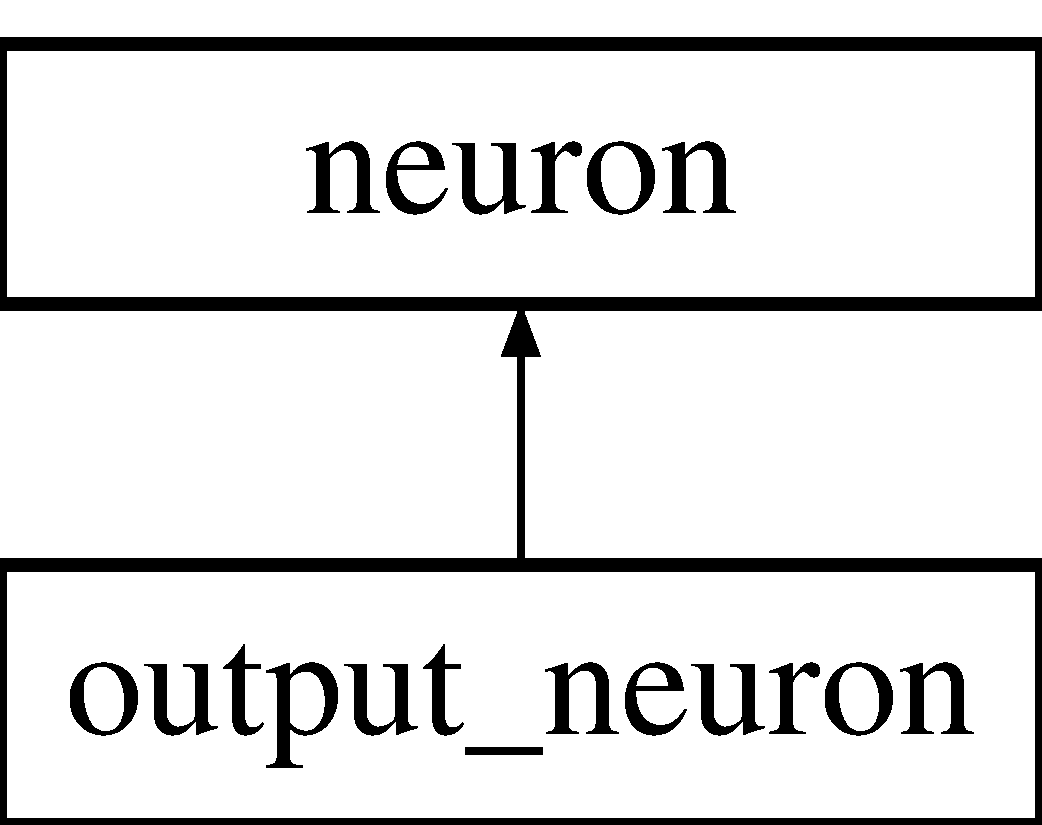
\includegraphics[height=2.000000cm]{classoutput__neuron}
\end{center}
\end{figure}
\subsection*{Public Member Functions}
\begin{DoxyCompactItemize}
\item 
\mbox{\Hypertarget{classoutput__neuron_a09856c092b517aee4f4aaa59e0ce8e02}\label{classoutput__neuron_a09856c092b517aee4f4aaa59e0ce8e02}} 
void \mbox{\hyperlink{classoutput__neuron_a09856c092b517aee4f4aaa59e0ce8e02}{calculate\+\_\+value}} () override
\begin{DoxyCompactList}\small\item\em Check if have any input axon before trying to calculate its output. If have none outputs 0. \end{DoxyCompactList}\end{DoxyCompactItemize}
\subsection*{Additional Inherited Members}


\subsection{Detailed Description}
Neuron that check if have any input axon before trying to calculate its output. If have none it outputs 0. 

Definition at line 59 of file neuron.\+h.



The documentation for this class was generated from the following files\+:\begin{DoxyCompactItemize}
\item 
backend/neural\+\_\+network/neuron.\+h\item 
backend/neural\+\_\+network/neuron.\+cpp\end{DoxyCompactItemize}

%--- End generated contents ---

% Index
\backmatter
\newpage
\phantomsection
\clearemptydoublepage
\addcontentsline{toc}{chapter}{Index}
\printindex

\end{document}
